\documentclass[a4paper,11pt]{article}
\usepackage[utf8]{inputenc}
\usepackage[swedish]{babel}
\usepackage{graphicx}
\usepackage[colorinlistoftodos]{todonotes}
\usepackage[affil-it]{authblk}
\usepackage{verbatim}
\usepackage{microtype}
\usepackage{amssymb}
\usepackage{tocloft}
\renewcommand{\cftsecleader}{\cftdotfill{\cftdotsep}}

\usepackage{animate}
\usepackage{amsthm}
\usepackage{hyperref}
\usepackage{gensymb}
\usepackage[hypcap=false]{caption}
\usepackage[version=4]{mhchem}
\usepackage[swedish]{babel}
\emergencystretch=1em
\usepackage[
backend=biber,
style=numeric,
sorting=none
]{biblatex}
\usepackage{color}
\usepackage{hyperref}
\hypersetup{colorlinks,citecolor=red,linkcolor=red}

\begin{document}

\begin{titlepage}
	\centering
	
\includegraphics[width=0.6\textwidth]{Bilder/logo.png}\par\vspace{1cm}
	\vspace{1.5cm}
	{\huge\bfseries Internetshistoria\par}
	\vspace{2cm}
	{\Large\itshape Adam Blomberg\par}
	\vfill
\animategraphics[width=1\textwidth]{12}{Bilder/grandmaSurf/grandma-}{0}{18}
	\vfill

% Bottom of the page
	{\large \today\par}
\end{titlepage}

\tableofcontents
\newpage

\section{Där det hela började}

Det var tidigt 60-tal och Joseph Licklider hade redan storslagna planer om ett intergalaktiskt nätverk. Hans vision var ett globalt sammanlänkat nätverk av datorer som alla med tillgång till nätverket snabbt skulle kunna hämta data och program från alla webbsidor. Man skulle kunna säga att han var mycket före sin tid eftersom att hans vision sedan blev verklighet under 2000-talet. Syftet var att skapa ett säkert och decentraliserat nätverk som inte kunde slås ut av något främmande främmande land, främst Sovjetunionen. Arpanet skapades av den amerikanska forskningsanstalten \textit{Advanced Research Projects Agency,} ARPA år 1969. Det fanns endast en omfattande aktör inom  telekombranchen vilket var AT\&T som nästan hade monopol, de ägde telefonledningarna som så småningom om skulle komma att användas till att koppla ihop datorerna i ARPANET. Universitetet UCLA i Kaliforninen skickade det första meddelandet vilket var kommandot "LOG", som skulle användas för att fjärrlogga in på en annan dator. Mottagardatron krashade dock innan den hunnit ta emot hela kommandot, meddelandet som skickades blev istället "LO". Det är en historisk händelse då datorer för första gången har pratat med varandra.

På tal om Sovjet, de hade en liknande ide. Kort därefter att J. Licklider talat om sina tankar, börjar Viktor Glushkov berätta om sin liknande plan med namnet OGAS. Detta går att jämnföra med Rymdkapplöpningen som ägde rum mellan 50- till 60-tal. Det var tänkt att OGAS skulle var uppdelat i tre lager, enligt Glushkov. Nätverket skulle ha sitt styre i Moskva med totalt 20.000 sammankopplade datorer genom Sovjetunionen. Datan skulle passera genom det redan existerande telefonledningarna på en frekvens som då inte var utnyttjad av telefonsamtalen, men ju mer data som behöver passera genom telefonledningarna desto större behöver frekvensspannet att vara. Till en viss punkt kan du inte göra spannet större och du har då kommit till en slutpunkt. Under denna tid var inte detta ett stort problem, men med tiden började vi ladda ned mer och strömma video. Det är därför fiber används istället nu för tiden eftersom att den har mycket större bandbredd.

{\centering
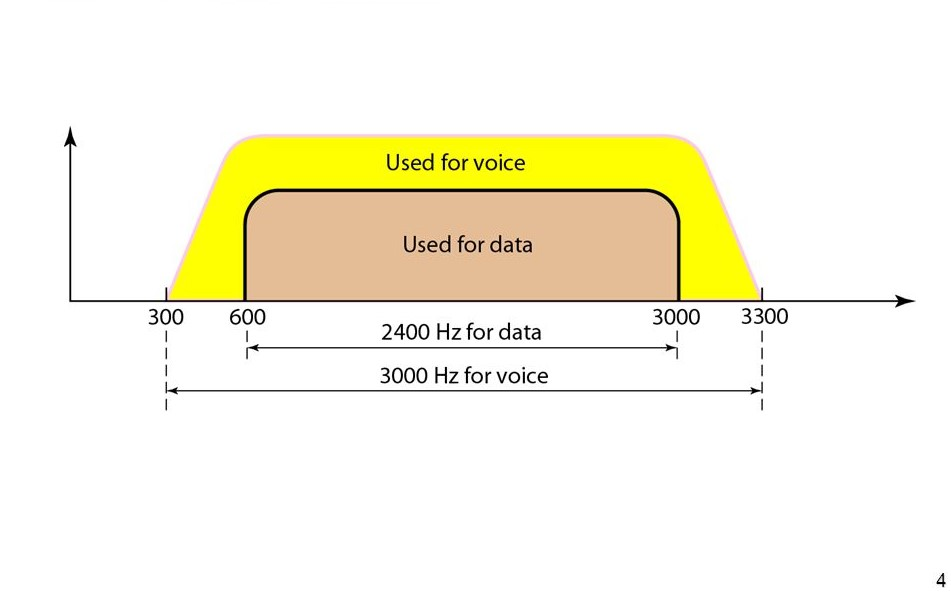
\includegraphics[width=1\linewidth]{Bilder/bandbredd.jpg}
\captionof{figure}{Som vi kan se i denna illustration används majoriteten av bandbredden i telefonledningarna till data överföring vilket omfattar faxmedelanden, men främst internetanvänding.}
} \newpage

Tanken var att de skulle kunna kommunicera med varandra på en decentraliserad nivå -- utan att behöva passera genom Moskva. Det var senare tänkt att under etapp två -- skulle resterande världen anslutats, främst Europa och Asien. USA var inte ens på kartan på grund av de dåliga relationerna mellan Sovietunionen och USA. Alla fabriker och kontorskomplex skulle vara uppkopplat. Det var en genialisk idé enligt Glushkov själv. Genom nätverket skulle framförallt betalningar ske digitalt, ungefär som det sker idag via internetbankerna.

Projektet blev dock aldrig en verklighet eftersom att Glushkov inte lyckades finansiera sitt projekt, han fick inte vidare finansiering av regeringen. Vid det laget har Arpanet redan slagit rot, som senare kommer att bli det vi idag kallar internet. Det var först 1969 som det första meddelandet skickades på Arapanet.
\end{document}
